\documentclass[10pt]{beamer}

%% Chinese support
\usepackage[adobefonts,nocap]{ctex}


\usepackage{amsmath}

\usepackage{natbib}

\usepackage{hyperref}

%% Fonts
\usepackage{multicol}
%\usepackage{mathabx}
%\usepackage[scaled]{helvet}
%\usepackage{lmodern}
%\usepackage{eulervm}
%\usefonttheme[onlymath]{serif}
%\usefonttheme{professionalfonts}
%\usefonttheme{structurebold}
\usepackage{bm}
\usepackage{verbatim}

%% Color & Theme
\definecolor{SUblue}{RGB}{0,0,180}
\usecolortheme[RGB={0,0,180}]{structure}
\usetheme{Boadilla}
\setbeamertemplate{navigation symbols}{}
\setbeamertemplate{itemize items}[circle]
\setbeamertemplate{enumerate items}[circle]
\setbeamerfont{title}{size=\large}
\setbeamerfont{frametitle}{size=\large}
\setbeamerfont{framesubtitle}{size=\large,shape =$\color{violet}{\looparrowdownright}~$}
\setbeamercolor{title}{fg=white, bg= SUblue!75!green}
\setbeamercolor{framesubtitle}{fg=violet}
%\setlength{\leftmargini}{30pt}


\title[High Performance Computing with Big Data]{{\textbf{大规模数
      据Logistic回归}}}

\subtitle{---基于GPU和高效内存技术的快速计算}

\author[马景义~李丰~孙志猛~王汉生]{\\马景义$^1$~李丰$^1$~孙志
  猛\footnote{中央财经大学统计与数学学院} ~王汉生\footnote{北京大学光华
    管理学院}}

\institute[]{\includegraphics[height=2cm]{cufelogo}
\includegraphics[height=2cm]{pkulogo}}

\date{五月22日·腾讯}

\begin{document}

%% Title page
\begin{frame}[plain]
  \titlepage
  \tiny{Rev: \today}
\end{frame}


%% Outline page
\section*{~}
\begin{frame}
  \frametitle{~}
  \tableofcontents
\end{frame}

\section{大数据下复杂模型面临挑战}
\begin{frame}
  \frametitle{背景}

  \begin{itemize}


  \item 因为大数据:

    \begin{itemize}
    \item 所以Hadoop/Mapreduce, Spark,...

    \item 所以数据更复杂,要求复杂模型,但是复杂模型在大数据平台实现并
      不容易。
    \end{itemize}
  \item 传统的统计学家/数据科学家:

    \begin{itemize}
    \item 知道许多复杂模型

    \item 但是只能在个人电脑(小于32G内存)上操作。
    \end{itemize}

  \item 现有工具

    \begin{itemize}
    \item 一个中等偏上的计算机基本配置(约1万RMB):32G内存,独立显卡,1-2T硬盘。
    \item R/Python等语言提供了主流统计模型的in-memory的基本实现,但是慢!
    \item 底层语言C/C++有对数据读写的memory-effcient方法,但是不适合直
      接拿来作复杂模型的统计计算。
    \end{itemize}

  \end{itemize}

\end{frame}


\begin{frame}
  \frametitle{大数据下复杂模型面临挑战}

  % \begin{itemize}
  % \item 看起来是一个非常简单的方法,但是做好不容易。
    \begin{itemize}

    \item 复杂模型估计需要通过复杂迭代算法实现。

      \begin{itemize}
      \item 迭代算法特有的依赖性使得模型估计很难被并行。
      \item 全数据的迭代算法不可行。
      \end{itemize}

    \item 各个击破策略:合理对数据分块然后分别估计,最后汇总。

      \begin{itemize}
      \item 如何分块影响到模型估计的准确度,以线性回归为例 \citet{ma2013statistical}


      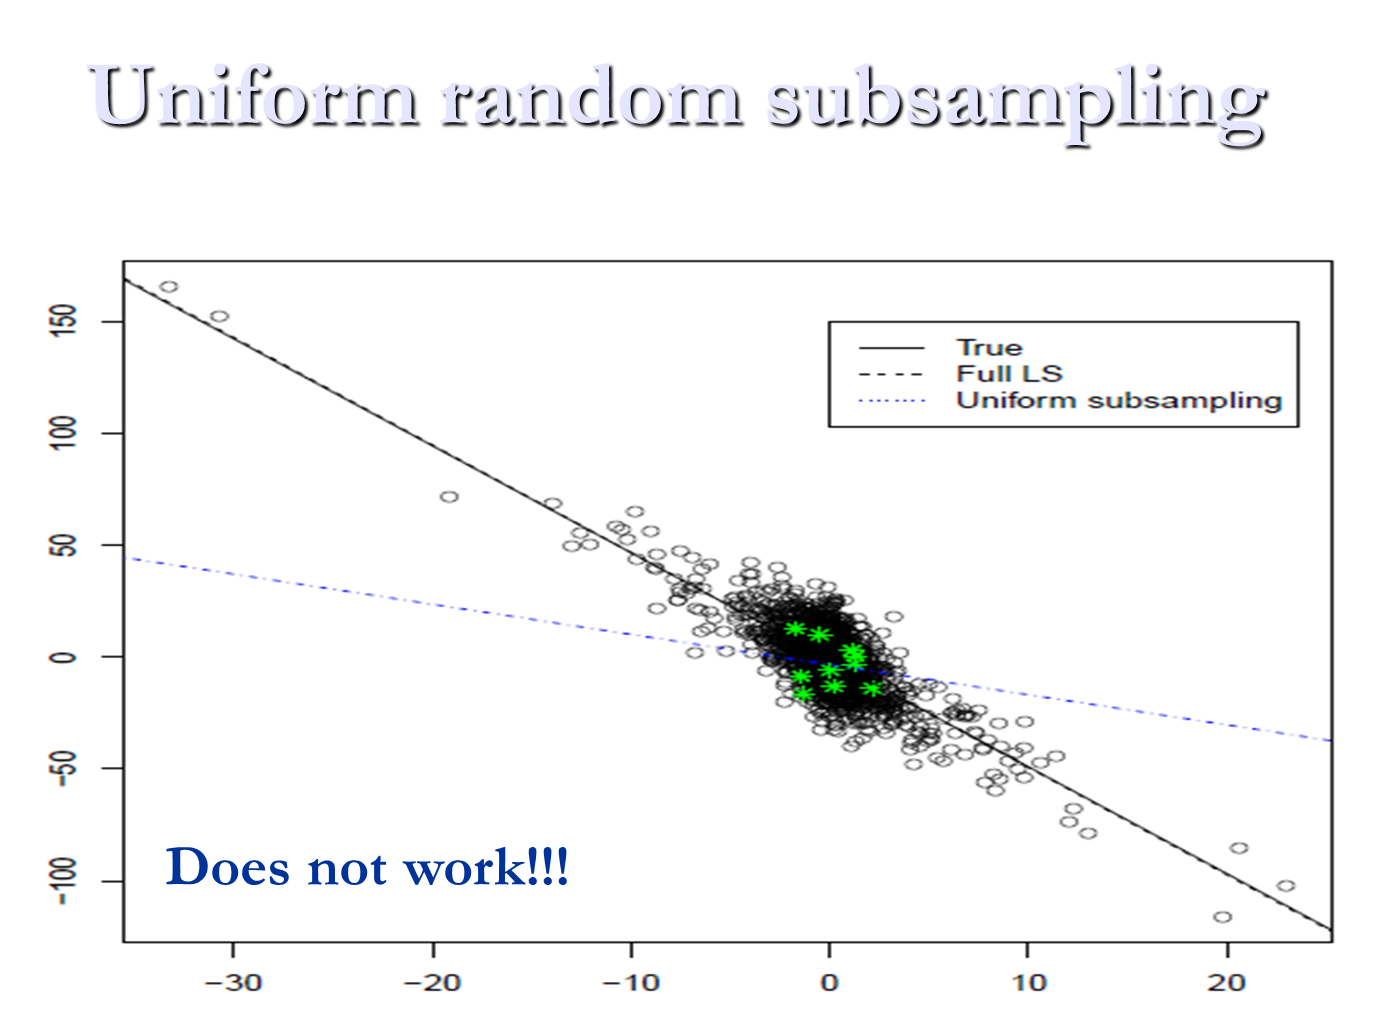
\includegraphics[trim=2cm 0.3cm 0cm 4cm,clip,width=0.6\textwidth]{leverage}


    \item 理论上讲分块方法并没有降低计算的复杂度。但是提高单个分块模型的计算性
      能变得可能。

      \end{itemize}

    \end{itemize}

  % \end{itemize}

\end{frame}


\begin{frame}
  \frametitle{各个击破: 以Logistic回归为例}
  \includegraphics[trim= 1.5cm .5cm 1.2cm 0.5cm, clip,
  height=0.8\textheight]{divide-and-conquer}
\end{frame}



\section{基于GPU的分块 Logistic 回归模型}

\begin{frame}
  \frametitle{工作流程}
  \includegraphics[trim= 1.5cm 3.5cm 1.2cm 1cm, clip,
  height=0.8\textheight]{workflow}
\end{frame}


\begin{frame}
  \frametitle{理论支撑}

  \begin{itemize}
  \item Logistic 回归模型

    \begin{equation*}
      p(y_i) = \frac{\exp\{x_i'\beta\}}{1+\exp\{x_i'\beta\}}
    \end{equation*}

    其中 $x_i=(x_{i1},...,x_{ip})'$, $i=1,...,n$。 利用极大似然估计可以
    得到 $\beta$ 的估计值,$\widehat \beta$。

  \item 分块 Logistic 回归模型

    \begin{itemize}
    \item 把 $n$ 个样本分为 $k$ 块,每块包含 $m$ 个观测值。
    \item 对于每一块数据作Logistic 回归得到
      \begin{equation*}
        \widehat \beta_l = \arg~\max \sum _{i =1}^m \{ y_{li}x_{li}'\beta-\log(1+\exp\{x_i'\beta\})\}.
      \end{equation*}

    \item 全部样本的Logistic回归模型的估计量$\widehat \beta$可以利用分
      块Logistic回归模型 $\widehat \beta_l$ 加权得到
      \begin{equation*}
        \widehat \beta = \frac{1}{k}\sum_{l=1}^k \widehat \beta_l.
      \end{equation*}
    \end{itemize}

  \end{itemize}


\end{frame}

\begin{frame}
  \frametitle{一些极限性质}

当$m \to \infty$, $n \to \infty$,可以证明
  \begin{itemize}
  \item 相合性:
    \begin{equation*}
      {\widehat \beta} \xrightarrow{p} \beta.
    \end{equation*}

  \item 渐近正态性:
    \begin{equation*}
      \sqrt{n} (\widehat \beta -\beta) \sim N(0, I(\beta))
    \end{equation*}
    其中

    \begin{equation*}
      I(\beta) = \lim \limits_{m \to \infty} \frac{1}{k}\sum_{l=1}^k
      \{\frac{1}{m}\sum_{i=1}^m var (s(\beta_l))\}^{-1}.
\end{equation*}


  % \item 更多关于 divide and conquer 方法的理论性质参见 Jordan(2012,
  %   KDD)。

  \end{itemize}
\end{frame}




\begin{frame}
  \frametitle{工作测试环境}

  \begin{itemize}

  \item 32G 内存,128G SSD,2T 物理硬盘
  \item Tesla C2050显卡: 448 CUDA Cores, 3GB total dedicated Memory

    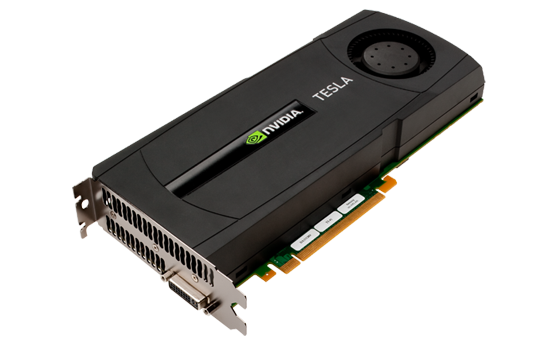
\includegraphics[width=0.4\textwidth]{tesla}


  \item 软件环境:Debian Linux (64-bit), CUDA toolkit, Intel Compiler,
    LAPACK, BLAS。

  \item 用户终端界面:R

  \end{itemize}

\end{frame}



  \begin{frame}
    \frametitle{Bottom necks \& Speedups}

    \begin{itemize}


    \item 分块数据虽然可以读到内存中已经占用较多内存,很难继续
      进行数据计算。

      \begin{center}
        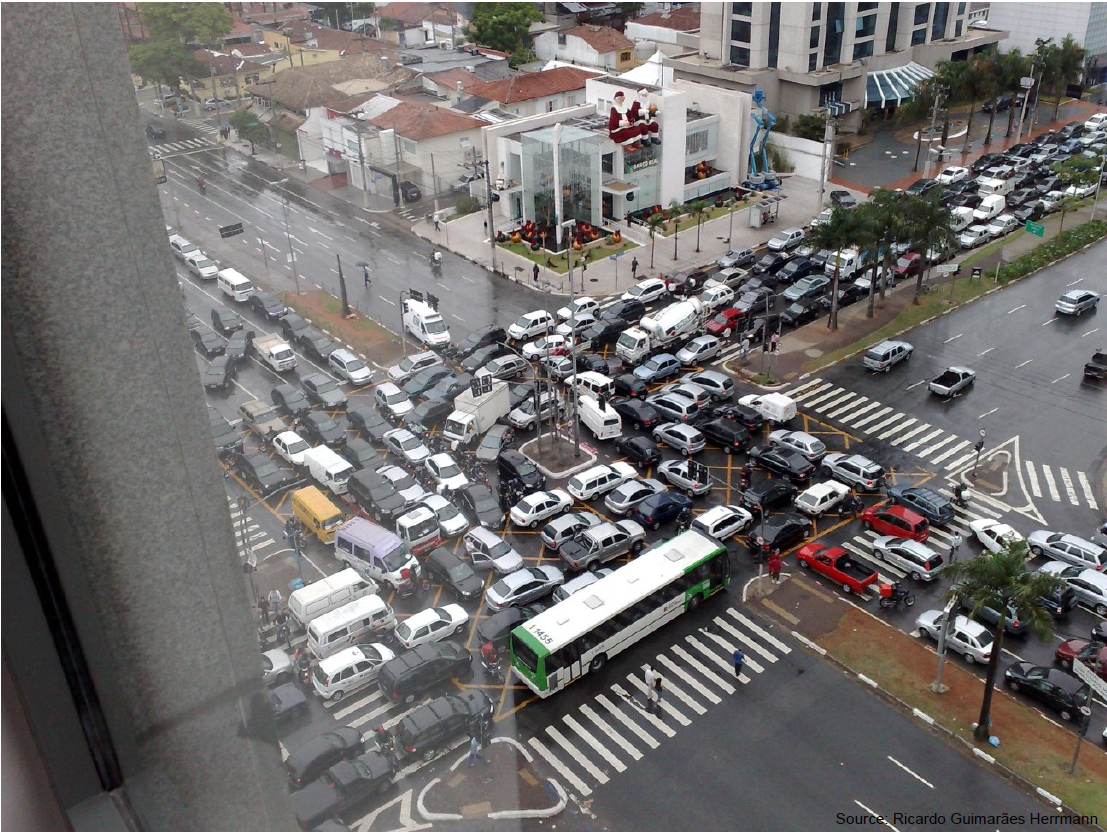
\includegraphics[width=0.6\textwidth]{memory-jam}
      \end{center}

    \item Memory-efficient R内存管理(C++实现Transparent memory
      mapping, \citet{kane2010scalable})

 \end{itemize}

  \end{frame}



  \begin{frame}
    \frametitle{Bottom necks \& Speedups}

    \begin{itemize}

    \item 将Logistic回归分解,80\%时间用来计算对数据矩阵$X'X$的QR分解。

    \item 利用GPU可以将QR分解提速290倍以上\citep{tomov2010dense}。

      \centering
      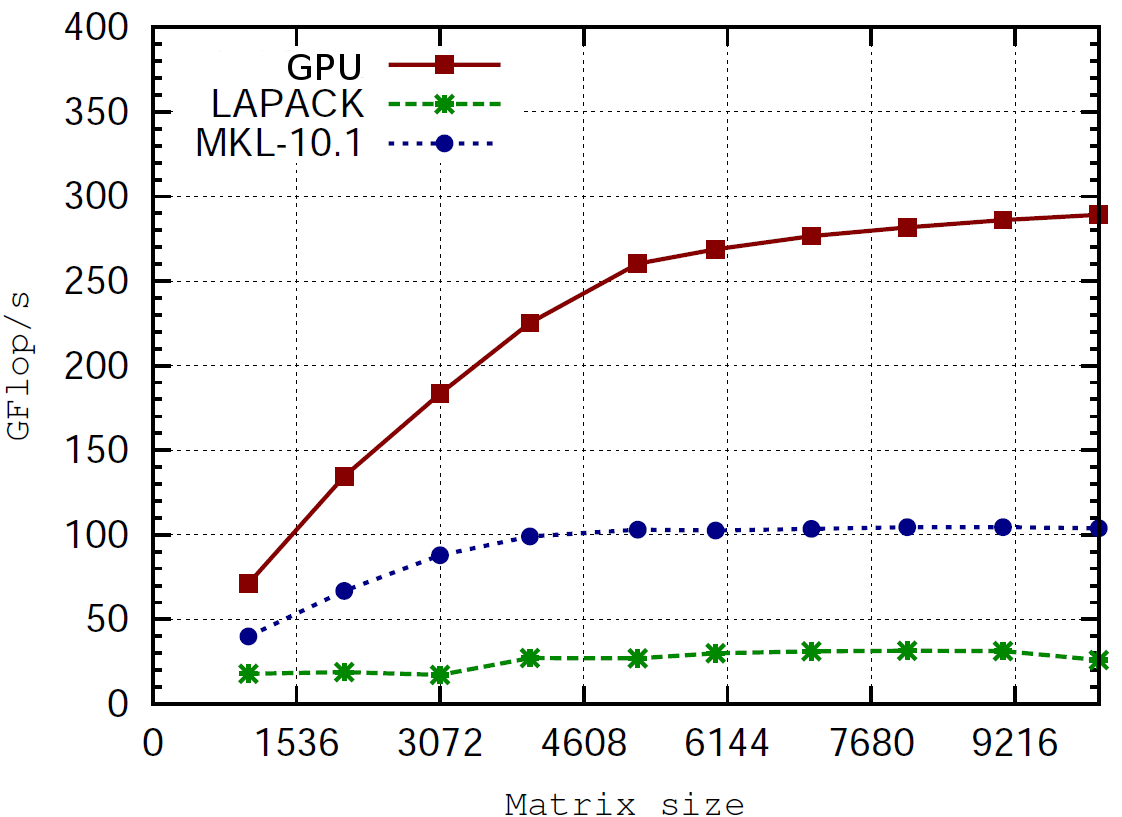
\includegraphics[width=0.6\textwidth]{QR}

 \end{itemize}

  \end{frame}


\section{扩展}

\begin{frame}
  \frametitle{扩展性}

  \begin{itemize}

  \item 实现机制可以理解为单机版的MapReduce,但不仅仅是MapReduce。

  \item 方法具有一般性,可以拓展到一般的统计分类模型。
  \item 方法可以方便的部署到并行计算集群,进行超大规模统计模型的快速计算。

  \end{itemize}

\end{frame}

  \begin{frame}
    \frametitle{参考文献}

    %\begin{small}
    %\phantomsection
    %\addcontentsline{toc}{section}{\bibname}
    \def\newblock{\hskip .11em plus .33em minus .07em} % important line
    \bibliographystyle{asa}
    \bibliography{full,References}
    % \end{small}

  \end{frame}


\begin{frame}


  \begin{center}
   \color{blue}{\Huge 谢谢!}
  \end{center}

  %\centering
  %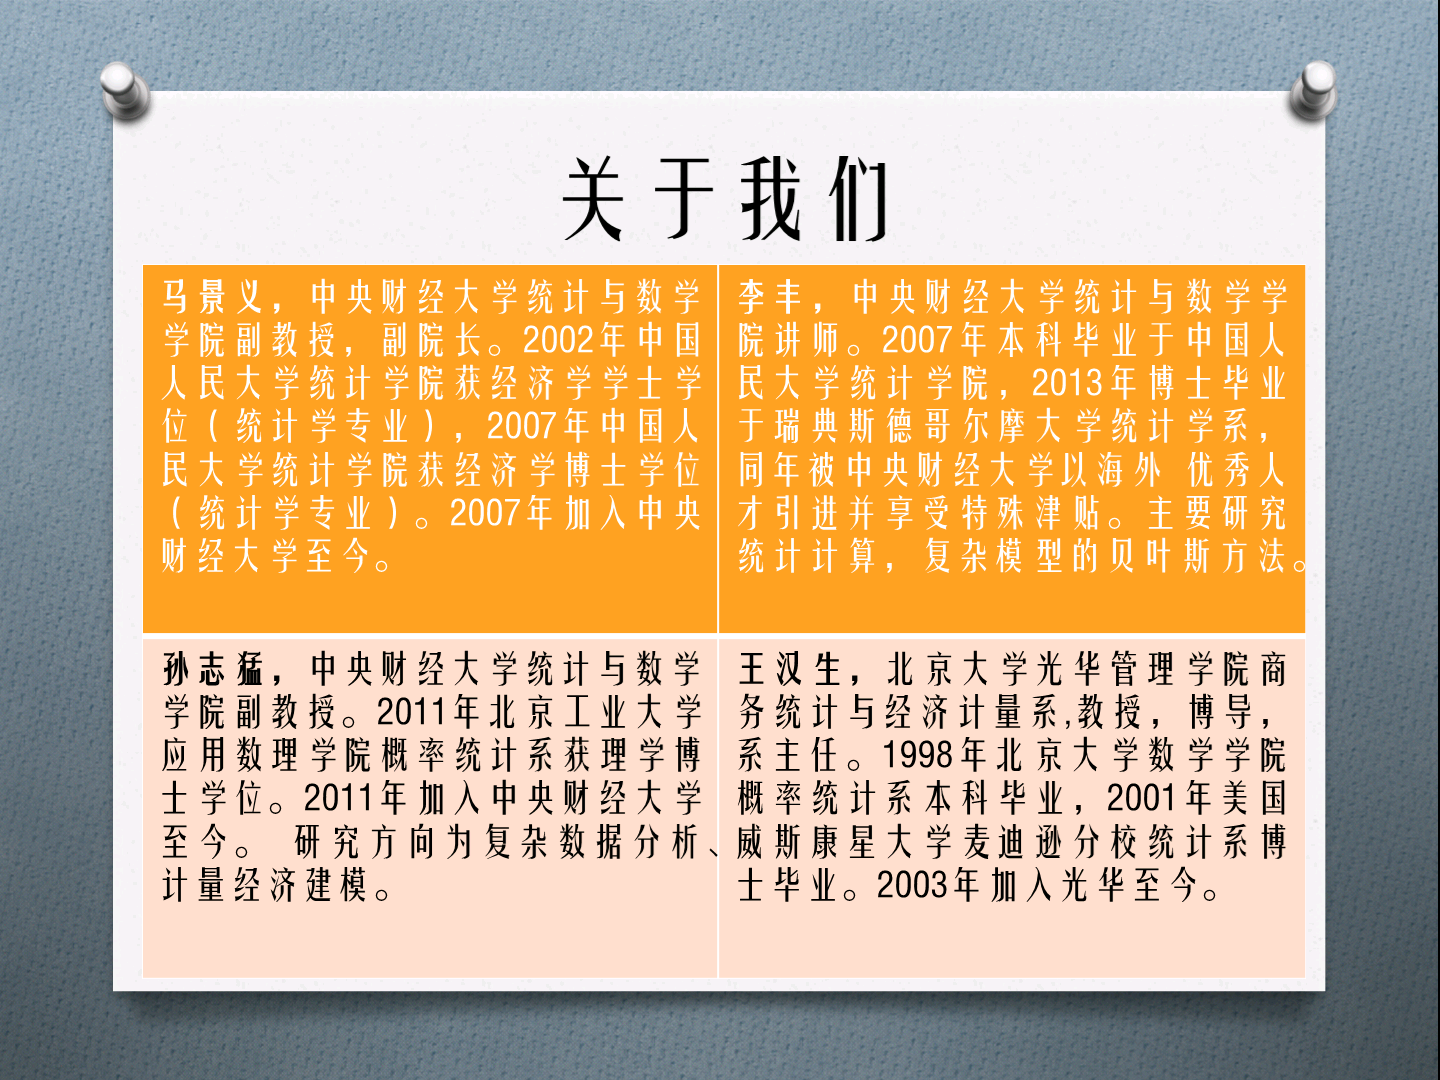
\includegraphics[height=0.7\textheight]{authors}

\end{frame}

\end{document}
